\documentclass[11pt]{article}
\usepackage[T1]{fontenc}
\usepackage{lmodern}
\usepackage[margin=1in]{geometry}
\usepackage{amsmath,amssymb,amsthm,mathtools}
\usepackage{microtype}
\usepackage{booktabs}
\usepackage{tikz}
\usepackage[numbers,sort&compress]{natbib}
\usepackage[colorlinks=true,linkcolor=blue,citecolor=blue,urlcolor=blue]{hyperref}
\ifdefined\pdfinfoomitdate\pdfinfoomitdate=1\fi
\ifdefined\pdftrailerid\pdftrailerid{}\fi
\ifdefined\pdfsuppressptexinfo\pdfsuppressptexinfo=15\fi
\newcommand{\HH}{\mathcal H}
\newcommand{\IMM}{\operatorname{IMM}}
\newcommand{\C}{\mathbb C}
\newcommand{\N}{\mathbb N}
\newcommand{\Z}{\mathbb Z}
\newcommand{\Q}{\mathbb Q}
\newcommand{\e}{\mathrm e}
\DeclareMathOperator{\rank}{rank}
\DeclareMathOperator{\tr}{tr}
\DeclareMathOperator{\dist}{dist}
\newtheorem{theorem}{Theorem}[section]
\newtheorem{lemma}[theorem]{Lemma}
\newtheorem{proposition}[theorem]{Proposition}
\newtheorem{corollary}[theorem]{Corollary}
\theoremstyle{definition}
\newtheorem{definition}[theorem]{Definition}
\theoremstyle{remark}
\newtheorem{remark}[theorem]{Remark}

\title{Homogeneous depth-five lower bounds for iterated matrix multiplication}
\author{OpenAI}
\date{September 25, 2026}
\hypersetup{pdftitle={Homogeneous depth-five lower bounds for iterated matrix multiplication},pdfauthor={OpenAI}}
\begin{document}
\maketitle
\begin{abstract}
Let $\IMM_{n,n}$ be the $(1,1)$ entry of a product of $n$ independent
$n\times n$ matrices of variables. Over every field of characteristic zero,
every syntactically homogeneous $\Sigma\Pi\Sigma\Pi\Sigma$ circuit
computing $\IMM_{n,n}$ has at least $n^{\sqrt n/400}$ gates for all
sufficiently large $n$, with an absolute threshold independent of the field.
Bottom linear forms may have arbitrary support, and arbitrary finite
fan-in, fan-out, and gate sharing are allowed. Over every field, a block
expansion gives such circuits with at most $n^{\sqrt n+4}$ gates for $n\geq2$.
Thus the gate complexity over characteristic-zero fields is
$n^{\Theta(\sqrt n)}$.
\end{abstract}
\tableofcontents
\section{Introduction}
\label{sec:introduction}

We study how many gates are needed to compute iterated matrix multiplication
with five homogeneous arithmetic layers.  For integers $w,d\geq 1$, let
$X^{(1)},\ldots,X^{(d)}$ be $w\times w$ matrices whose entries are distinct
commuting variables.  Define
\begin{equation}
\label{eq:imm-definition}
 \IMM_{w,d}
 =\bigl(X^{(1)}\cdots X^{(d)}\bigr)_{1,1}
 =\sum_{i_1,\ldots,i_{d-1}\in[w]}
   x^{(1)}_{1,i_1}x^{(2)}_{i_1,i_2}\cdots x^{(d)}_{i_{d-1},1}.
\end{equation}
For $d=1$, the expression means $x^{(1)}_{1,1}$.  The first index denotes
matrix width and the second denotes degree.  We retain all $dw^2$ matrix-entry
variables as ambient variables, including entries absent from the polynomial.
Our target is $\IMM_{n,n}$, of degree $n$ in $n^3$ ambient variables.

\subsection{Circuit model and main result}

An arithmetic circuit over a field $K$ is a finite directed acyclic graph.
Its leaves are variables or elements of $K$.  A sum gate computes a
$K$-linear combination of its inputs, and a product gate computes their
product.  Fan-in and fan-out are arbitrary and finite.  Gates may be shared,
and a gate may occur repeatedly among another gate's inputs; repeated
occurrences at a product gate are counted with their multiplicities.
Scalar coefficients on sum inputs are part of the circuit and do not require
additional gates.

A $\Sigma\Pi\Sigma\Pi\Sigma$ circuit has five computational layers,
listed from output to leaves, with respective gate types
$+,\times,+,\times,+$ and a single output gate.  Edges between computational
gates join consecutive layers, and the bottom sums read leaves.  Unary gates
are allowed.  In particular, no bound is placed on the number of variables
in a bottom linear form.

The circuit is \emph{syntactically homogeneous} if it has the following
formal-degree assignment: variables have degree $1$, constants have degree
$0$, product gates add their input degrees with multiplicity, and all inputs
of a sum gate have the same degree, which is assigned to that gate.  Empty
sums and products, if present, compute $0$ and $1$ and have formal degree $0$.
Thus a zero polynomial at a gate still carries its assigned formal degree;
cancellation does not reset that degree.  All computations and equalities
below concern formal polynomials.

We define \emph{size} to be the number of vertices, including leaves.  The
number of computational gates excludes leaves, whereas wire size counts
input occurrences.  These quantities are not identified: our lower bound is
on gates, and the circuit analysis also bounds the number of computational
gates alone.

\begin{theorem}
\label{thm:main}
There exist absolute constants $c>0$ and $n_0$ such that, for every integer
$n\geq n_0$, every syntactically homogeneous
$\Sigma\Pi\Sigma\Pi\Sigma$ circuit over $\C$ computing $\IMM_{n,n}$
has size at least
\[
 n^{c\sqrt n}.
\]
One may take $c=1/400$.
\end{theorem}

The model permits unrestricted bottom fan-in and support, constants, and
shared subcircuits.  Corollary~\ref{cor:characteristic-zero} extends the
$n^{\sqrt n/400}$ lower bound to every field of characteristic zero, with
the same absolute threshold.  Proposition~\ref{prop:upper} gives an
elementary block construction of size at most $n^{\sqrt n+4}$ over every
field for $n\geq2$.  It is homogeneous of depth four; inserting unary bottom
sums makes it depth five, so the lower bound has the matching scale.
Iterated matrix multiplication nevertheless has polynomial-size circuits
when depth is unrestricted.

\subsection{Historical context and previous bounds}

Iterated matrix multiplication has long served as a test of the cost of
restricting arithmetic depth.  Its path expansion connects matrix products
with reachability, while its polynomial-size unrestricted circuits make it
a natural target for lower bounds on weaker circuit models.
Nisan and Wigderson used dimensions of partial-derivative spaces to prove
lower bounds for homogeneous depth-three circuits and for constant-depth
set-multilinear circuits.  They asked for an explicit homogeneous polynomial
requiring superpolynomial size at constant depth, even at depth five
\cite[Section~2.2 of the linked author journal manuscript]{NisanWigderson1995}.

Depth reduction gave this program a further motivation.
Agrawal and Vinay reduced general arithmetic computation to depth four,
and Koiran and Tavenas sharpened the size bounds
\cite{AgrawalVinay2008,Koiran2012,Tavenas2013}.
For $d=N^{O(1)}$, Tavenas's theorem converts a circuit of size
$N^{O(1)}$ computing a homogeneous degree-$d$ polynomial in $N$ variables
to a homogeneous depth-four circuit of size $N^{O(\sqrt d)}$
\cite[Theorem~1 of the linked preprint]{Tavenas2013}.
This explains the square-root scale in depth-four lower bounds and in the
block construction for IMM used here.

The progress toward this scale involved several distinct restrictions.
Fournier, Limaye, Malod, and Srinivasan proved
IMM lower bounds with bounds on both product-layer fan-ins and, separately,
for homogeneous multilinear formulas
\cite[Theorems~16 and~29 of the cited author version]{FournierLimayeMalodSrinivasan2015}.
Kayal, Limaye, Saha, and Srinivasan removed the bottom-fan-in restriction
for homogeneous depth-four formulas, obtaining an exponential lower bound
over characteristic zero for a Nisan--Wigderson design family
\cite[Theorem~1]{KayalLimayeSahaSrinivasan2014}.
Kumar and Saraf proved a $d^{\Omega(\sqrt d)}$ lower bound for homogeneous
depth-four circuits computing $\IMM_{d^5,d}$, over every field
\cite[Theorem~1.2 and Section~8.2 of the cited preprint]{KumarSaraf2014}.
In another direction, Kayal, Saha, and Tavenas obtained
$w^{\Omega(\sqrt d)}$ for syntactically multilinear depth-four circuits
computing $\IMM_{w,d}$, without homogeneity, in the range
$d\geq\log^2 w$, over every field
\cite[Theorem~1.4 and the following comparison]{KayalSahaTavenas2018}.

At depth five, Bera and Chakrabarti proved a lower bound with a restriction
on bottom support.
Their Theorem~1.1 states that, for every fixed $0\leq\mu<1/2$, there is
an integer $q=q(\mu)>0$ such that homogeneous
$\Sigma\Pi\Sigma\Pi\Sigma$ circuits computing $\IMM_{d^q,d}$, with
$N=d^{2q+1}$ ambient variables and bottom fan-in at most $N^\mu$, require
$N^{\Omega_\mu(\sqrt d)}$ gates over every field
\cite[Theorem~1.1]{BeraChakrabarti2015}.
Their precise Theorem~4.2 proves the lower bound for a restricted IMM
polynomial, using the number of distinct variables feeding each bottom
linear gate as its support parameter
\cite[Theorem~4.2]{BeraChakrabarti2015}.
The Kumar--Saraf and Bera--Chakrabarti bounds use different width--degree
regimes from $w=d=n$, and the latter restricts the bottom linear forms.

For a different hard family, Kumar and Saptharishi proved, over each fixed
finite field $\mathbb F_q$,
$\exp(\Omega_q(\sqrt d))$ lower bounds for homogeneous depth-five circuits
without a bottom-support restriction
\cite[Theorem~1]{KumarSaptharishi2017}.
Their family is based on Nisan--Wigderson designs and lies in
$\mathrm{VNP}$.
Armand, Behera, and Tavenas have since extended this finite-field approach
to depth-five circuits whose top-product fan-in is bounded by a fixed
polynomial in the degree $d$, without homogeneity
\cite[Corollary~1.3]{ArmandBeheraTavenas2026}.
These finite-field theorems concern NW polynomials rather than IMM; both
the field hypothesis and the exponential rate differ from those in
Theorem~\ref{thm:main}.

Superpolynomial lower bounds for unrestricted-bottom depth-five circuits
over characteristic zero were already established by the constant-depth
results of Limaye, Srinivasan, and Tavenas
\cite{LimayeSrinivasanTavenas2021,LimayeSrinivasanTavenas2025}.
We use the theorem numbering of their ECCC revision~1.
Their product-depth convention counts multiplication gates on a path, so
our five-layer model has product-depth two.  In the low-degree regime
$d\leq(\log w)/100$, their Corollary~3 gives
$w^{\Omega(\sqrt d)}$ for homogeneous product-depth-two circuits over every
field~\cite[Corollary~3]{LimayeSrinivasanTavenas2021}.
Their general-circuit results also imply superpolynomial lower bounds for
$\IMM_{n,n}$ over $\C$
\cite[Corollary~4 and the following discussion]{LimayeSrinivasanTavenas2021}.
Bhargav, Dutta, and Saxena improved the constant-depth exponents in the
low-degree regime \cite{BhargavDuttaSaxena2022}.
Forbes subsequently established low-depth IMM lower bounds over arbitrary
fields in the regime $d=o(\log w)$~\cite[Theorem~10]{Forbes2024}.

Amireddy, Garg, Kayal, Saha, and Thankey gave a direct shifted-partials
approach.  For homogeneous product-depth-two formulas they obtain
$2^{-O(d)}w^{\Omega(\sqrt d)}$ when $w=\omega(d)$, over every field
\cite[Theorem~24]{AmireddyGargKayalSahaThankey2023}.
The degree-dependent loss and the hypothesis $w=\omega(d)$ prevent direct
substitution of $w=d=n$.  The comparison addressed here is quantitative:
we obtain the $\sqrt n$ exponent in the balanced regime $w=d=n$ for
homogeneous five-layer circuits with unrestricted bottom linear forms.

\subsection{Proof overview}

The proof uses a derivative-based linear-algebraic measure.  Dimensions of
partial-derivative spaces were used by Nisan and
Wigderson~\cite{NisanWigderson1995}; shifted partial derivatives were developed
in work of Kayal~\cite{Kayal2012} and Gupta, Kamath, Kayal, and
Saptharishi~\cite{GuptaKamathKayalSaptharishi2014}.
We define the operator needed here directly and prove its estimates.

Partition the matrix layers into two groups containing $k$ and $m$ layers,
where $k+m=n$ and $m-k$ is of order $\sqrt n$.  Let $V$ and $U$ be the
corresponding variable sets.  For a homogeneous polynomial $g$ of degree
$n$, let $g_{[k,m]}$ be the sum of its monomials having degree $k$ in $V$ and
degree $m$ in $U$.  Replace its $V$-variables by partial derivatives and
its $U$-variables by multiplication operators.  On polynomials of fixed
bidegree $(a,b)$ this gives a linear map
\[
 F_g=g_{[k,m]}(\partial_V,U)
\]
into polynomials of bidegree $(a-k,b+m)$.  We choose $a,b$ of order
$n^{5/2}$, write $D$ for the dimension of the source, and use
$R(g)=\rank F_g$ as the complexity measure.  Differentiation in $V$ commutes
with multiplication in $U$; the full substitution therefore respects
products, while the finite map is linear in $g$ and its rank is subadditive.
Section~\ref{sec:rank} gives the definitions and parameters.

We first bound the rank of a circuit in Section~\ref{sec:circuits}.
For a product of homogeneous factors, resolve each factor into its possible
$V$-degrees.  Apply first those factors whose $V$-degree exceeds their
proportional share $ke/n$ for a factor of degree $e$.  Their composition passes through
a smaller intermediate polynomial space, which bounds its rank.  The
distance of each proportional share from the integers controls the sum over
all such decompositions.  These are the same integer-degree discrepancies
that underlie the residue method of Amireddy, Garg, Kayal, Saha, and
Thankey \cite[Definition~2.1 and Lemma~3.1]{AmireddyGargKayalSahaThankey2022Full};
here they control intermediate homogeneous dimensions.
If all factor degrees are small, these distances
give the required saving.  If some factor has large degree, expand just one
such factor into its bottom products of linear forms.  This costs at most
one additional factor of the circuit size.  Proposition~\ref{prop:circuit}
gives, for a size-$S$ circuit,
\[
 R(g)\leq 2S^2D\exp(C\sqrt n)\,n^{-\sqrt n/100}
\]
with an absolute constant $C$.

The opposite estimate uses the paths in matrix multiplication.
Section~\ref{sec:moments} arranges the two groups of layers in a balanced
order, with no adjacent $V$-layers.  Declare the monomials
$z^M/\sqrt{M!}$ orthonormal, where $M$ is an exponent vector and
$M!$ is the product of its coordinate factorials.  In these bases,
differentiation and multiplication have coefficients given by square roots
of exponents and their successors.  For $g=\IMM_{n,n}$,
the first two trace moments of $F_g^*F_g$ become weighted counts of paths
and quadruples of paths.  Exact factorial moments for uniform weak
compositions compare these weights with independent geometric random
variables.  We verify the coefficient signs needed for that comparison.

At each layer, a contributing quadruple has one of two pairing patterns.
A change of pattern forces four vertex labels to agree and reduces the
number of choices by a factor of $n$.  Section~\ref{sec:path-sum} sums the
resulting weights, treating isolated corrections and the two endpoints
explicitly.  The balanced order controls the weight accumulated along each
run of one pattern.  The trace inequality
\[
 \rank H\geq\frac{(\tr H)^2}{\tr(H^2)}
 \qquad(H\ne0\text{ positive semidefinite})
\]
then yields $R(\IMM_{n,n})\geq D\exp(-C'\sqrt n)$, as stated in
Proposition~\ref{prop:imm}.  Section~\ref{sec:completion} compares the two
rank estimates and proves the field extension and matching upper bound.

\section{A rank measure from differentiation and multiplication}
\label{sec:rank}

We associate a linear map to a polynomial by differentiating in one
group of variables and multiplying in a disjoint group.  The rank of
this map is subadditive.  More importantly, the map associated to a
product can be factored through intermediate homogeneous spaces, whose
dimensions will control the circuit upper bound.

\subsection{The operator and its homogeneous spaces}

Let $K$ be a field, and let $V,U$ be disjoint finite sets of variables,
of cardinalities $v,u\ge1$.  For a variable set $E$ and an integer
$t\ge0$, write $\HH_E(t)=K[E]_t$ for the vector space of homogeneous
polynomials of degree $t$.  Its dimension is
\[
 h(|E|,t),\qquad h(r,t)=\binom{r+t-1}{t}.
\]
For $Q\in K[V,U]$, let
\[
 T_Q=Q(\partial_V,U)
\]
be the operator on $K[V,U]$ obtained by replacing each variable in $V$
by its formal partial derivative and each variable in $U$ by
multiplication by that variable.  These operators commute because the
two variable sets are disjoint.  Thus $T_{Q_1Q_2}=T_{Q_1}T_{Q_2}$.
This identity holds over every field.

Fix integers $k,m\ge0$, $a\ge k$, and $b\ge0$.  If $g$ is homogeneous
of degree $k+m$, denote its component of $V$-degree $k$ and $U$-degree
$m$ by $g_{[k,m]}$.  Define the finite-dimensional map
\begin{equation}
\label{eq:rank-map}
 F_g=g_{[k,m]}(\partial_V,U):
 \HH_V(a)\otimes\HH_U(b)
 \longrightarrow
 \HH_V(a-k)\otimes\HH_U(b+m),
 \qquad R(g)=\rank F_g.
\end{equation}
The source dimension is $D=h(v,a)h(u,b)$.  Projection to a bidegree
and operator substitution are both linear, so
\[
 R(g_1+g_2)\le R(g_1)+R(g_2),\qquad
 R(cg)=R(g)\quad(c\in K\setminus\{0\}).
\]
Also $R(0)=0$.  The multiplicative identity for $T_Q$ does not assert
multiplicativity of $g\mapsto F_g$: the latter includes a fixed
bidegree projection.  We will first decompose products into their
bidegree components and then use multiplicativity of $T_Q$ on each
contribution.

\subsection{Choosing the degrees}

We now choose the spaces in~\eqref{eq:rank-map} for degree-$n$
polynomials on the $n$ matrix layers.  Throughout the proof $n$ is
sufficiently large, and all implicit constants and thresholds are
absolute.  Let $s$ be the largest integer at most $\sqrt n$ having the
same parity as $n$, and put
\begin{equation}
\label{eq:parameters}
\begin{gathered}
 k=\frac{n-s}{2},\qquad m=\frac{n+s}{2},\qquad
 \rho=\frac{k}{m},\qquad \lambda=\frac{k}{n}
       =\frac{\rho}{1+\rho},\\
 v=kn^2,\qquad u=mn^2,\qquad
 a=\left\lceil\frac{v}{\sqrt n-1}\right\rceil,
 \qquad \alpha=\frac{a}{a+v},\\
 b=\left\lceil\frac{u\alpha^\rho}{1-\alpha^\rho}\right\rceil,
 \qquad \beta=\frac{b}{b+u},\qquad
 q=\alpha^{(1+\rho)/2},\qquad D=h(v,a)h(u,b).
\end{gathered}
\end{equation}
For now assign any $k$ full matrix layers to $V$ and the other $m$
layers to $U$.  Each layer retains all its $n^2$ variables, including
variables absent from the endpoint entry of the matrix product.
Section~\ref{sec:moments} will specify their order when bounding the
rank of $\IMM_{n,n}$ from below.

The small excess $m-k=s$ makes the slope $\lambda$ slightly less than
$1/2$.  For small positive even factor degrees $e$, this moves
$\lambda e$ away from the integers; Section~\ref{sec:circuits}
quantifies the resulting rank saving.  The definitions of $a,b$
balance the dimension decrease caused by differentiation against the
dimension increase caused by multiplication.  Without the ceiling in
the definition of $b$, we would have $\beta=\alpha^\rho$ and
$\alpha^k\beta^{-m}=1$.  We record the rounding estimates explicitly,
as their errors must stay small after many factors are combined.

\begin{lemma}
\label{lem:parameters}
For all sufficiently large $n$, the parameters in~\eqref{eq:parameters}
satisfy
\begin{gather*}
 \frac{\sqrt n}{2}\le s\le\sqrt n,\qquad
 \lambda\ge\frac38,\qquad 0<\rho<1,\qquad
 v,u=\Theta(n^3),\qquad a,b=\Theta(n^{5/2}),\\
 a\ge k,\qquad 2n\le\frac12\min(a,b),\qquad
 n^{-1/2}\le\alpha=n^{-1/2}\exp(O(1/a)),\qquad
 \alpha^{-1}\le\sqrt n,\\
 \alpha^\rho\le\beta\le\alpha^\rho\exp(C/b),
 \qquad \beta\le\frac2{\sqrt n},\\
 q=n^{-1/2}\exp\bigl(O(s\log n/n+1/a)\bigr),
 \qquad n^{-1/2}\le q\le\frac2{\sqrt n}
 \le n^{-2/5},\qquad q\le\frac12,
\end{gather*}
where $C$ is an absolute constant.
\end{lemma}

\begin{proof}
The parity choice gives $\sqrt n-2<s\le\sqrt n$, and hence the
claims about $s,k,m,\lambda,\rho,v,u$.  Write
$a_0=v/(\sqrt n-1)$, so that $a_0\le a<a_0+1$ and
$a_0/(a_0+v)=n^{-1/2}$.  The function $x/(x+v)$ is increasing, and
the derivative of its logarithm is $v/(x(x+v))\le1/x$.
The mean value theorem therefore gives
\[
 0\le\log(\alpha n^{1/2})\le\frac1{a_0}=O(1/a).
\]
In particular $a=\Theta(n^{5/2})$ and $\alpha^{-1}\le\sqrt n$.

Since $1-\rho=s/m=O(s/n)$, the preceding estimate implies
\[
 \alpha^\rho
 =n^{-1/2}\exp\bigl(O(s\log n/n+1/a)\bigr)
 =n^{-1/2}(1+o(1)).
\]
Put $b_0=u\alpha^\rho/(1-\alpha^\rho)$.  Then
$b_0=\Theta(n^{5/2})$, $b_0\le b<b_0+1$, and
$b_0/(b_0+u)=\alpha^\rho$.  Applying the same logarithmic derivative
bound with $u$ in place of $v$ gives
\[
 0\le\log(\beta/\alpha^\rho)\le1/b_0\le C/b.
\]
This proves the assertions about $b,\beta$, including
$\beta\le2/\sqrt n$ eventually.  The growth of $a,b$ also gives
$a\ge k$ and $2n\le\min(a,b)/2$.

Finally,
\[
 \log q=-\frac{1+\rho}{4}\log n+O(1/a)
 =-\frac12\log n+O(s\log n/n+1/a).
\]
Because $0<\alpha<1$ and $(1+\rho)/2\le1$, we have
$q\ge\alpha\ge n^{-1/2}$.  The remaining upper bounds follow from
the last display and $s\log n/n\to0$.
\end{proof}

The estimate $q\le n^{-2/5}$ will suffice for the main power savings.
The sharper $q=O(n^{-1/2})$ will be essential when summing the
smaller errors contributed by even factor degrees.

\section{The rank of a homogeneous depth-five circuit}
\label{sec:circuits}

We now bound the rank measure in terms of circuit size.  The argument
is uniform over the choice of the $k$ matrix layers assigned to $V$.
Its first step bounds the rank of a product using only the degrees of
its factors.  We then expand one middle-layer sum when its degree is
large, exposing its lower products of linear forms.

\begin{proposition}
\label{prop:circuit}
There are absolute constants $C>0$ and $n_0$ with the following property.
For $n\ge n_0$, use the parameters in~\eqref{eq:parameters} and any
partition of the matrix layers with $k$ layers in $V$ and $m$ layers in
$U$.  Let $K$ be a field, and let $g\in K[V,U]$ be a homogeneous
degree-$n$ polynomial computed by a syntactically homogeneous
$\Sigma\Pi\Sigma\Pi\Sigma$ circuit of size $S$.  Then
\[
 R(g)\le 2S^2D\exp(C\sqrt n)\,n^{-\sqrt n/100}.
\]
\end{proposition}

All thresholds in this section are absorbed into a single absolute
$n_0$, independent of the field, the circuit, and the partition.
Only the parameter estimates of Lemma~\ref{lem:parameters} will be
used.

\subsection{Products and intermediate dimensions}

For a positive integer $e$, define
\[
 H_e=\sum_{i=0}^{e}q^{|i-\lambda e|}.
\]
These quantities account for all choices of bidegree in a product.

The quantities $H_e$ use the same integer-degree discrepancies as the
residue method of Amireddy, Garg, Kayal, Saha, and Thankey
\cite[Definition~2.1 and Lemma~3.1]{AmireddyGargKayalSahaThankey2022Full}.
In the present argument they control the dimensions of the intermediate
homogeneous spaces through which the differentiation--multiplication
operator factors.

\begin{lemma}
\label{lem:product-rank}
Let $K$ be a field, and let $Q_1,\ldots,Q_r\in K[V,U]$ be homogeneous of respective positive
degrees $e_1,\ldots,e_r$, with $\sum_{j=1}^r e_j=n$.  Then
\[
 R\left(\prod_{j=1}^r Q_j\right)
 \le 2D\prod_{j=1}^r H_{e_j}.
\]
\end{lemma}

\begin{proof}
Decompose each factor into its bidegree components.  The component of
their product that defines the rank measure is
\[
 \left(\prod_{j=1}^r Q_j\right)_{[k,m]}
 =\sum_{\substack{0\le i_j\le e_j\ (1\le j\le r)\\
                   \sum_j i_j=k}}
   \prod_{j=1}^r (Q_j)_{[i_j,e_j-i_j]}.
\]
Fix an assignment in this sum, and put
$\delta_j=i_j-\lambda e_j$.  Since $\lambda n=k$, we have
$\sum_j\delta_j=0$.  The operators obtained by substituting
$\partial_V$ and $U$ commute, so we may apply first the factors with
$\delta_j>0$.  Write their total bidegree as
\[
 I=\sum_{\delta_j>0}i_j,
 \qquad J=\sum_{\delta_j>0}(e_j-i_j).
\]
The resulting intermediate space is
$\HH_V(a-I)\otimes\HH_U(b+J)$.  It is well defined because
$I\le k\le a$; also $J\le m$.  Its dimension bounds the rank of this
contribution, including when the set of positive discrepancies is
empty.

The successive ratios of binomial coefficients give
\begin{align*}
 \frac{h(v,a-I)}{h(v,a)}
 &=\prod_{t=0}^{I-1}\frac{a-t}{a+v-1-t}
 \le\left(\frac{a}{a+v-1}\right)^I,\\
 \frac{h(u,b+J)}{h(u,b)}
 &=\prod_{t=1}^{J}\frac{b+u+t-1}{b+t}
 \le\left(\frac{b+u}{b}\right)^J
 =\beta^{-J}.
\end{align*}
The first inequality follows because $x/(x+v-1)$ is nondecreasing for
$x>0$.  Since $\beta\ge\alpha^\rho$, these inequalities imply
\begin{equation}
\label{eq:intermediate-dimension}
 \frac{h(v,a-I)h(u,b+J)}{D}
 \le \alpha^{I-\rho J}
       \left(1-\frac1{a+v}\right)^{-I}
 \le 2\alpha^{I-\rho J}.
\end{equation}
The last bound holds uniformly for $I\le n$, because
$a+v=\Theta(n^3)$.  Empty products in the ratio formulas equal 1.

Using $\lambda=\rho/(1+\rho)$ and $\sum_j\delta_j=0$, we obtain
\[
 I-\rho J
 =(1+\rho)\sum_{\delta_j>0}\delta_j
 =\frac{1+\rho}{2}\sum_j|\delta_j|.
\]
As $q=\alpha^{(1+\rho)/2}$, the rank of the fixed-assignment
contribution is therefore at most
\[
 2D\prod_j q^{|i_j-\lambda e_j|}.
\]
Rank subadditivity permits summing these bounds.  Dropping the
constraint $\sum_j i_j=k$ increases the resulting nonnegative sum
and makes it factor as $2D\prod_jH_{e_j}$.  Zero bidegree components
contribute rank zero throughout.
\end{proof}

\subsection{The cost of integer degrees}

The product estimate is effective because $\lambda e$ is usually
separated from the integers.  Small even degrees require particular
care: their separation can tend to zero, so a constant loss for each
factor would be too large.  We bound their combined error instead.

Put
\[
 d_e=\dist(\lambda e,\Z),\qquad t_0=\frac{n}{4s}.
\]
\begin{lemma}
\label{lem:degree-estimates}
For every integer $e\ge1$,
\begin{equation}
\label{eq:nearest-integer-bound}
 H_e\le q^{d_e}\bigl(1+4q^{1-2d_e}\bigr)\le5.
\end{equation}
If $1\le e<t_0$, then
\begin{equation}
\label{eq:low-degree-distances}
 d_e=
 \begin{cases}
   se/(2n),&e\text{ even},\\
   1/2-se/(2n),&e\text{ odd},
 \end{cases}
 \qquad d_e\ge\frac{se}{2n}.
\end{equation}
In this range, odd degrees satisfy $H_e\le q^{d_e/2}$, whereas even
degrees satisfy
\begin{equation}
\label{eq:even-degree-bound}
 H_e\le q^{d_e}\exp\bigl(4q^{1-se/n}\bigr).
\end{equation}
There is an absolute constant $C_1$ such that, for every finite list of
positive integers $e_1,\ldots,e_r$ with $\sum_j e_j\le n$,
\begin{equation}
\label{eq:even-corrections}
 \sum_{\substack{j:\ e_j<t_0\\ e_j\text{ even}}}
 q^{1-se_j/n}\le C_1\sqrt n.
\end{equation}
\end{lemma}

\begin{proof}
Enlarge the sum defining $H_e$ to all integers.  Apart from one nearest
integer to $\lambda e$, the terms have total at most
$2q^{1-d_e}/(1-q)$.  This remains valid when the nearest integer is
not unique.  Since $q\le1/2$, it gives the first inequality
in~\eqref{eq:nearest-integer-bound}; the second follows from
$0\le d_e\le1/2$ and $0<q<1$.

For $e<t_0$, write
\[
 \lambda e=\frac e2-\frac{se}{2n},
 \qquad 0<\frac{se}{2n}<\frac18.
\]
The nearest integer is consequently $e/2$ for even $e$, and
$(e-1)/2$ for odd $e$.  This proves
\eqref{eq:low-degree-distances}.  For odd $e$ we have $d_e\ge3/8$.
By $q\le n^{-2/5}$,
\[
 q^{-d_e/2}\ge n^{d_e/5}\ge n^{3/40}\ge5
\]
after increasing $n_0$.  Thus
$H_e\le5q^{d_e}\le q^{d_e/2}$.  For even $e$, substitute
$2d_e=se/n$ in~\eqref{eq:nearest-integer-bound} and use
$1+x\le\exp(x)$ to obtain~\eqref{eq:even-degree-bound}.

It remains to sum these even-degree errors.  Increase $n_0$ so that
$t_0>2$, and for real $z\in[2,t_0]$ define
\[
 f(z)=\frac{q^{1-sz/n}}{z}.
\]
Its logarithm is convex, since $(\log f)''(z)=1/z^2>0$.
Hence $f(z)\le\max\{f(2),f(t_0)\}$.  The sharp estimate for $q$ in
Lemma~\ref{lem:parameters} gives
\[
 f(2)
 =\frac12 n^{-1/2}
   \exp\bigl(O(s\log n/n+1/a)\bigr)
 =O(n^{-1/2}).
\]
At the other endpoint, $s\le\sqrt n$ and $q\le2n^{-1/2}$ give
\[
 f(t_0)=\frac{4s}{n}q^{3/4}=O(n^{-7/8}).
\]
Therefore $q^{1-se/n}\le C_1e/\sqrt n$ uniformly over the low even
degrees.  Summing and using $\sum_j e_j\le n$ proves
\eqref{eq:even-corrections}.
\end{proof}

These estimates control a product of factors below $t_0$ regardless
of their coefficients.  A factor of degree at least $t_0$ will instead
supply many linear factors through its bottom-layer expansion.

\subsection{From gates to products}

\begin{proof}[Proof of Proposition~\ref{prop:circuit}]
If $g=0$, the conclusion is immediate.  Otherwise its formal output
degree is $n$: induction on the gates shows that every nonzero
polynomial at a formally homogeneous degree-$d$ gate is homogeneous
of degree $d$.

We first record exactly what the circuit layers provide.  A bottom
sum gate computes either a homogeneous linear form or a scalar,
because all its leaf inputs have the same formal degree.  A lower
product of formal degree $e>0$ therefore computes a scalar times a
product of exactly $e$ homogeneous linear-form occurrences.
Degree-zero factors are absorbed into that scalar.  A zero factor
makes the whole product zero and its contribution can be discarded.
A gate computing zero need not be assigned a different formal degree.

At either a middle sum or the output sum, repeated wires from the
same predecessor gate can be combined by adding their scalar
coefficients.  There are at most $S$ distinct predecessors.  Thus
$g$ is a sum of at most $S$ scalar multiples of products
\begin{equation}
\label{eq:circuit-product-form}
 G=\prod_{j=1}^{r}Q_j,
 \qquad \deg Q_j=e_j\ge1,\qquad \sum_j e_j=n,
\end{equation}
and each $Q_j$ is a sum of at most $S$ scalar multiples of products
of $e_j$ homogeneous linear forms.  Zero upper terms have been
discarded, and degree-zero factors in the remaining terms have been
absorbed into their coefficients.  If empty sums or products are allowed, they
contribute only zero or a scalar and are handled in the same way.

In~\eqref{eq:circuit-product-form}, inputs to a product are counted
with multiplicity: repeated use of a gate gives repeated factors.
Their positive degrees add to $n$, so $r\le n$.  Shared subcircuits
do not affect the bounds on the number of distinct additive
predecessors.  In particular, this description does not charge for
wires or impose any restriction on the support of a linear form.

Suppose first that every $e_j<t_0$.  By
\eqref{eq:low-degree-distances},
\[
 \sum_j d_{e_j}\ge\frac{s}{2n}\sum_j e_j=\frac s2.
\]
Apply Lemmas~\ref{lem:product-rank} and~\ref{lem:degree-estimates},
weakening $q^{d_{e_j}}$ to $q^{d_{e_j}/2}$ for even degrees.  The
combined even-degree correction is at most $\exp(4C_1\sqrt n)$.
Consequently
\begin{equation}
\label{eq:all-low-product}
 R(G)\le2D\exp(4C_1\sqrt n)q^{s/4}
 \le2D\exp(4C_1\sqrt n)n^{-\sqrt n/20},
\end{equation}
where we used $q\le n^{-2/5}$ and $s\ge\sqrt n/2$.

Now suppose that one factor occurrence has degree $e\ge t_0$.
Expand that occurrence, using its middle sum, into at most $S$
products of $e$ homogeneous linear forms.  All other factors remain
unexpanded.  This includes any other occurrences of the same gate:
expanding one occurrence in $Q^h$ leaves its other $h-1$ occurrences
unexpanded.

In each resulting product, the $e$ newly supplied linear factors
contribute $H_1^e\le q^{\lambda e/2}$ to the estimate of
Lemma~\ref{lem:product-rank}, because $d_1=\lambda$ and $1<t_0$.
There are at most $n/t_0=4s$ remaining factor occurrences of degree
at least $t_0$, and their $H$-factors are at most 5 each.  The
remaining low odd degrees contribute at most 1.  The remaining low
even degrees contribute at most $\exp(4C_1\sqrt n)$ after their
favorable powers of $q$ are dropped.  Rank subadditivity over the
expansion therefore yields
\begin{align}
\label{eq:one-high-product}
 R(G)
 &\le2SD\,5^{4s}\exp(4C_1\sqrt n)q^{\lambda t_0/2}\notag\\
 &\le2SD\,5^{4s}\exp(4C_1\sqrt n)n^{-3\sqrt n/160}.
\end{align}
For the last step, $q\le n^{-2/5}$ and
$\lambda\ge3/8$, $t_0\ge\sqrt n/4$ imply
$\lambda t_0/5\ge3\sqrt n/160$.

Since $5^{4s}\le\exp(4\log(5)\sqrt n)$, both
\eqref{eq:all-low-product} and~\eqref{eq:one-high-product} are at most
\[
 2SD\exp(C\sqrt n)n^{-\sqrt n/100}
\]
for an absolute $C$.  Multiplication by a nonzero scalar leaves rank
unchanged, and multiplication by zero gives rank zero.  Summing the
at most $S$ upper-product contributions proves the proposition.
\end{proof}

\section{Trace moments for iterated matrix multiplication}
\label{sec:moments}

We now choose the partition of the layers and prove that its mixed operator
has large rank on iterated matrix multiplication.  The parameters remain
those of~\eqref{eq:parameters}.  Arrange the groups along the matrix product
in the order
\begin{equation}
  VU^{\ell_1}\,VU^{\ell_2}\cdots VU^{\ell_k},
  \qquad
  \ell_i=1+\left\lfloor\frac{is}{k}\right\rfloor
             -\left\lfloor\frac{(i-1)s}{k}\right\rfloor.
  \label{eq:balanced-schedule}
\end{equation}
For sufficiently large $n$ we have $0<s/k<1$, so each $\ell_i$ is either
one or two.  Their sum is $k+s=m$.  Thus this word has exactly $k$ layers
in $V$ and $m$ in $U$, and no two $V$ layers are adjacent.  Every layer
contributes all its $n^2$ variables to its group, including the variables
of the first and last matrices that do not occur in the $(1,1)$ entry.

Put $f=\IMM_{n,n}$ and $L=n-1$.  A path $P$ is a sequence
$(p_0,\ldots,p_n)$ with $p_0=p_n=1$ and $p_1,\ldots,p_{n-1}\in[n]$.
Its coordinate in layer $t$ is
\[
  E_t(P)=x^{(t)}_{p_{t-1},p_t}.
\]
There are $n^L$ paths, and $f$ is the sum of the products of their layer
coordinates.  In particular, $f$ has bidegree $(k,m)$, so its finite map
$F_f$ is the restriction of the full operator $T_f=f(\partial_V,U)$ to
$\HH_V(a)\otimes\HH_U(b)$.

\begin{proposition}
\label{prop:imm}
Over $\C$, for the partition~\eqref{eq:balanced-schedule}, there is an
absolute constant $C$ such that, for all sufficiently large $n$,
\[
  R(\IMM_{n,n})\ge D\exp(-C\sqrt n).
\]
\end{proposition}

The proof uses two trace moments.  Give every homogeneous polynomial
space the inner product in which
\[
  \frac{z^M}{\sqrt{M!}},\qquad |M|=t,
  \qquad M!=\prod_i M_i!,
\]
is an orthonormal basis.  This is the finite homogeneous part of the
Bargmann--Fock polynomial normalization~\cite{Bargmann1962}.
Use the tensor product of these inner products
for the domain and codomain of $F_f$, and write
\[
  T=\tr(F_f^*F_f),\qquad
  T_2=\tr\bigl((F_f^*F_f)^2\bigr).
\]
If $T>0$, Cauchy--Schwarz applied to the nonzero eigenvalues of
$F_f^*F_f$ gives
\begin{equation}
  R(f)\ge \frac{T^2}{T_2}.
  \label{eq:trace-rank}
\end{equation}
Define
\[
  A=\frac av,\qquad B=\frac bu,\qquad
  \mu=A^k(1+B)^m.
\]
We will prove the bounds
\[
 T\ge Dn^L\mu\exp(-O(n^{-1/2})),\qquad
 T_2\le Dn^{2L}\mu^2\exp(O(\sqrt n)).
\]
This section reduces
the second bound to a sum over two-letter words; the next section bounds
that sum and completes Proposition~\ref{prop:imm}.

\subsection{Occupation moments}

A uniformly chosen basis vector of $\HH_V(a)\otimes\HH_U(b)$ has two
independent exponent vectors: one is uniform among weak compositions
of $a$ into $v$ parts, and the other among weak compositions of $b$
into $u$ parts.  We compare their moments with those of independent
geometric variables.  For an integer $d\ge0$, write
\[
  (z)_d=z(z-1)\cdots(z-d+1),\qquad
  r^{\overline d}=r(r+1)\cdots(r+d-1),
\]
with both empty products equal to one.

\begin{lemma}
\label{lem:occupation-moments}
Let $M=(M_1,\ldots,M_r)$ be uniform among the weak compositions of an
integer $t\ge0$ into $r\ge1$ parts.  For integers $d_i\ge0$ and
$H=\sum_i d_i$,
\begin{equation}
  \mathbb E\prod_i(M_i)_{d_i}
   =\frac{(t)_H}{r^{\overline H}}\prod_i d_i!.
  \label{eq:composition-moment}
\end{equation}
The right side is zero when $H>t$.

Let $Z_1,\ldots,Z_r$ be independent geometric variables on the
nonnegative integers with mean $G=t/r$.  If a polynomial $P$ has
nonnegative coefficients in the basis
$\{\prod_i(z_i)_{d_i}\}$, then
\begin{equation}
  \mathbb E P(M)\le\mathbb E P(Z).
  \label{eq:occupation-upper}
\end{equation}
If $t>0$ and all terms of that expansion have total order at most
$H_0\le t/2$, then also
\begin{equation}
  \mathbb E P(M)
  \ge
  \exp\left(-\frac{H_0^2}{t}-\frac{H_0^2}{2r}\right)
  \mathbb E P(Z).
  \label{eq:occupation-lower}
\end{equation}
\end{lemma}

\begin{proof}
For $d\ge0$,
\[
  \sum_{j\ge0}(j)_d y^j=\frac{d!y^d}{(1-y)^{d+1}}.
\]
If $H\le t$, coefficient extraction therefore gives
\[
  \sum_{|M|=t}\prod_i(M_i)_{d_i}
    =\left(\prod_i d_i!\right)
       \binom{t+r-1}{t-H}.
\]
Divide by $\binom{t+r-1}{t}$ to obtain
\eqref{eq:composition-moment}.  If $H>t$, every composition has
$M_i<d_i$ for some $i$, so every summand is zero, as is $(t)_H$.

For $G>0$, the geometric law is
\[
  \Pr(Z_i=j)=\frac1{1+G}\left(\frac{G}{1+G}\right)^j
  \quad(j\ge0),
\]
and its factorial moment is $\mathbb E(Z_i)_d=d!G^d$.  For $H\le t$
the ratio of the moment in~\eqref{eq:composition-moment} to the
corresponding independent geometric moment is
\begin{equation}
  \prod_{j=0}^{H-1}\frac{1-j/t}{1+j/r}.
  \label{eq:occupation-ratio}
\end{equation}
It is at most one.  For $H>t$ the composition moment is zero, so the
same upper comparison holds.  When $H\le H_0\le t/2$, the inequalities
$\log(1-x)\ge-2x$ for $0\le x\le1/2$ and
$\log(1+x)\le x$ for $x\ge0$ show that the logarithm of
\eqref{eq:occupation-ratio} is at least
\[
  -\sum_{j=0}^{H-1}\left(\frac{2j}{t}+\frac{j}{r}\right)
  \ge -\frac{H_0^2}{t}-\frac{H_0^2}{2r}.
\]
Sum these comparisons with the nonnegative coefficients of $P$.
If $t=0$, both $M$ and the geometric vector of mean zero are identically
zero, giving~\eqref{eq:occupation-upper} directly.
\end{proof}

The comparison is termwise and does not assert independence of the
coordinates of $M$.  We apply it separately in the two groups.
By Lemma~\ref{lem:parameters}, total orders at most $2n$ satisfy the
lower-bound hypothesis, and their combined logarithmic loss is
\begin{equation}
  O\left(\frac{n^2}{a}+\frac{n^2}{v}
          +\frac{n^2}{b}+\frac{n^2}{u}\right)
  =O(n^{-1/2}).
  \label{eq:occupation-loss}
\end{equation}

\subsection{The first trace}

In the chosen orthonormal bases, differentiation and multiplication
act by
\[
  \partial_i\frac{z^M}{\sqrt{M!}}
    =\sqrt{M_i}\frac{z^{M-\mathbf e_i}}{\sqrt{(M-\mathbf e_i)!}},
  \qquad
  z_i\frac{z^M}{\sqrt{M!}}
    =\sqrt{M_i+1}\frac{z^{M+\mathbf e_i}}{\sqrt{(M+\mathbf e_i)!}}.
\]
The derivative is zero when $M_i=0$; its displayed expression is used
only when $M_i\ge1$.  Here $\mathbf e_i$ is the coordinate unit vector.
In particular, repeated differentiation of order $d$ has coefficient
$\sqrt{(M_i)_d}$, with no additional factorial divisor.

Index a domain basis vector by the combined exponent vector $M$ on
$V\cup U$, with totals $a$ and $b$ in the two groups.  The summand of
$F_f$ corresponding to a path $P$ shifts this vector by
\[
  \epsilon_P
  =-\sum_{t:\,V}\mathbf e_{E_t(P)}
    +\sum_{t:\,U}\mathbf e_{E_t(P)}
\]
with coefficient
\begin{equation}
  c_P(M)
    =\left(
       \prod_{t:\,V}M_{E_t(P)}
       \prod_{t:\,U}(M_{E_t(P)}+1)
      \right)^{1/2}.
  \label{eq:path-coefficient}
\end{equation}
A shift requiring a negative occupation contributes zero.  We extend
the coefficient notation by zero to invalid input indices as well.
Different layers have disjoint coordinates, so a path never repeats a
coordinate.  Moreover, the shifts $\epsilon_P$ are distinct: a shift
specifies the coordinate in every layer and hence every vertex of $P$.

Consequently different paths from the same input reach different
output indices.  Summing the squared entries of $F_f$ gives the exact
identity
\[
  T=D\sum_P\mathbb E\left[
       \prod_{t:\,V}M_{E_t(P)}
       \prod_{t:\,U}(M_{E_t(P)}+1)
      \right],
\]
where the expectation is over the uniform domain indices.  Every
polynomial inside this expectation has nonnegative falling-factorial
coefficients.  Under independent geometric occupations of means $A$
and $B$, its expectation is $\mu$.  Lemma~\ref{lem:occupation-moments}
and~\eqref{eq:occupation-loss} therefore imply
\begin{equation}
  T\ge Dn^L\mu\exp(-O(n^{-1/2}))>0.
  \label{eq:first-trace}
\end{equation}
The inactive endpoint coordinates are included in the uniform
compositions and in $v,u$ throughout; they introduce no additional
factor into this calculation.

\subsection{Four paths in the second trace}

The matrix entries of $F_f$ in these bases are real and nonnegative.
An entry of $F_f^*F_f$ indexed by $M,M'$ is the sum of
$c_P(M)c_Q(M')$ over pairs of paths satisfying
$M+\epsilon_P=M'+\epsilon_Q$.  Squaring its entries and summing yields
\begin{equation}
\begin{split}
  T_2
   &=D\,\mathbb E_M
      \sum_{\substack{P,Q,R,S:\
        \epsilon_P-\epsilon_Q=\epsilon_R-\epsilon_S}}
        c_P(M)c_Q(M')c_R(M)c_S(M'),\\[-2pt]
  &\hspace{34mm} M'=M+\epsilon_P-\epsilon_Q.
\end{split}
  \label{eq:four-path-trace}
\end{equation}
The zero convention handles invalid indices.  There is no additional
sum over $M'$, because $M,P,Q$ determine it.

The condition on four paths holds separately in each layer.  Denoting
their four coordinates in that layer by $p,q,r,s$, respectively, it is
$\mathbf e_p-\mathbf e_q=\mathbf e_r-\mathbf e_s$.  If this difference
is zero, then $p=q$ and $r=s$.  Otherwise its positive and negative
coordinates force $p=r$ and $q=s$, with $p\ne q$.  Thus there are exactly
two types:
\[
\begin{array}{c|l}
  \mathcal N & p=q=i,\quad r=s=j,\\
  \mathcal D & p=r=i,\quad q=s=j,\quad i\ne j.
\end{array}
\]
The all-equal case belongs to $\mathcal N$.  For each compatible
quadruple, the four-coefficient product in~\eqref{eq:four-path-trace}
is a product over layers of the following polynomials:
\begin{equation}
\begin{array}{c|cc}
  &\mathcal N&\mathcal D\\ \hline
  V&M_iM_j&M_i(M_j+1)\\
  U&(M_i+1)(M_j+1)&(M_i+1)M_j.
\end{array}
  \label{eq:local-polynomials}
\end{equation}
Indeed, the shift from $M$ to $M'$ is zero in type $\mathcal N$.
In a $V$ layer of type $\mathcal D$ it is $-\mathbf e_i+\mathbf e_j$,
so the two coefficients at $M$ contribute $M_i$ and the two at $M'$
contribute $M_j+1$.  In a $U$ layer of type $\mathcal D$ the shift is
$\mathbf e_i-\mathbf e_j$, giving $(M_i+1)M_j$ instead.

These polynomial formulas also account for invalid indices.  In type
$\mathcal D$, a negative coordinate of $M'$ requires $M_i=0$ in a $V$
layer or $M_j=0$ in a $U$ layer, and the corresponding table entry
vanishes.  In type $\mathcal N$, an unavailable derivative makes
$M_iM_j$ zero.  Since different layers use distinct coordinates, these
exhaust the possible failures.  Thus the product in
\eqref{eq:local-polynomials} equals the zero-extended contribution.

When $i=j$ in type $\mathcal N$, the required expansions are
\[
  z^2=(z)_2+(z)_1,
  \qquad
  (z+1)^2=(z)_2+3(z)_1+1.
\]
All other table entries are products of $(z)_1$ and $(z)_1+1$ on distinct
coordinates.  Hence every product of local entries has nonnegative
falling-factorial coefficients, with order at most $2k$ in $V$ and
$2m$ in $U$.  Lemma~\ref{lem:occupation-moments} bounds its expectation
by the expectation for independent geometric occupations.

For a geometric variable $Z$ of mean $G$,
$\mathbb EZ^2=2G^2+G$ and
$\mathbb E(Z+1)^2=2G^2+3G+1$.  Dividing the geometric expectations in
each $V$ layer by $A^2$ and in each $U$ layer by $(1+B)^2$, we obtain
\begin{equation}
\begin{array}{c|cc}
  &\mathcal N&\mathcal D\\ \hline
  V&1+\alpha^{-1}\mathbf1_{\{i=j\}}&\alpha^{-1}\\
  U&1+\beta\mathbf1_{\{i=j\}}&\beta.
\end{array}
  \label{eq:local-weights}
\end{equation}
Here $(A+1)/A=\alpha^{-1}$ and $B/(B+1)=\beta$.  For example,
the repeated-coordinate $V$ entry is
$(2A^2+A)/A^2=1+\alpha^{-1}$, so the repeated factorial contribution
has been retained.  The product of the normalizing factors over all
layers is $\mu^2$.

\subsection{A sum over pairing types}

Assign to a compatible quadruple its type word
$\tau\in\{\mathcal N,\mathcal D\}^n$.  For each such word, enlarge its
class of quadruples by dropping the inequalities $i\ne j$ at all
$\mathcal D$ layers.  Keep their weights equal to $\alpha^{-1}$ and
$\beta$ as in~\eqref{eq:local-weights}.  These are assigned weights on
the newly admitted tuples, not their geometric occupation moments.
Every original tuple retains its weight, and every new weight is
nonnegative, so this enlargement gives an upper bound.

Equality of matrix-entry coordinates equates the path labels at both
ends of that layer.  The relaxed equalities can therefore be counted
independently at every internal vertex.  A layer of type $\mathcal N$
pairs the paths as
$\{P,Q\},\{R,S\}$, while a layer of type $\mathcal D$ pairs them as
$\{P,R\},\{Q,S\}$.  At a vertex between layers of the same type, there
are two free labels in $[n]$.  At a vertex between different types the
two pairings together identify all four labels, leaving one free label.
These give $n^2$ and $n$ choices, respectively, as illustrated in
Figure~\ref{fig:pairings}.
The two external vertex labels are fixed to $1$.  Every independent
choice at the internal vertices gives four paths, because all matrix
entries are available, and every relaxed quadruple arises uniquely
this way.  The set of assignments is therefore a Cartesian product
over internal vertices.  If
\[
  w(\tau)=\#\{t\in\{1,\ldots,n-1\}:\tau_t\ne\tau_{t+1}\},
\]
the number of assignments is exactly $n^{2L-w(\tau)}$.

\begin{figure}[tbp]
\centering
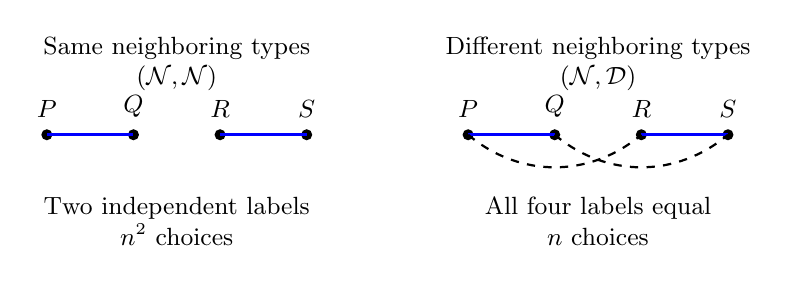
\begin{tikzpicture}[x=1cm,y=1cm,every node/.style={font=\small}]
  \node[align=center] at (1.65,1.65) {Same neighboring types\\($\mathcal N,\mathcal N$)};
  \node[align=center] at (7.0,1.65) {Different neighboring types\\($\mathcal N,\mathcal D$)};
  \foreach \x/\name in {0/P,1.1/Q,2.2/R,3.3/S,5.35/P,6.45/Q,7.55/R,8.65/S} {
    \fill (\x,0.75) circle (2pt);
    \node[above] at (\x,0.85) {$\name$};
  }
  \draw[very thick,blue] (0,0.75) -- (1.1,0.75);
  \draw[very thick,blue] (2.2,0.75) -- (3.3,0.75);
  \draw[very thick,blue] (5.35,0.75) -- (6.45,0.75);
  \draw[very thick,blue] (7.55,0.75) -- (8.65,0.75);
  \draw[thick,dashed] (5.35,0.75) to[bend right=40] (7.55,0.75);
  \draw[thick,dashed] (6.45,0.75) to[bend right=40] (8.65,0.75);
  \node[align=center] at (1.65,-0.35) {Two independent labels\\$n^2$ choices};
  \node[align=center] at (7.0,-0.35) {All four labels equal\\$n$ choices};
\end{tikzpicture}
\caption{Equality constraints on the four path labels at one internal
vertex after the $\mathcal D$ inequalities are relaxed.  Type $\mathcal N$ pairs $P,Q$
and $R,S$ (solid edges); type $\mathcal D$ pairs $P,R$ and $Q,S$ (dashed edges).
Equal neighboring types leave two free labels.  A change of type
identifies all four, contributing a factor $n^{-1}$ to the count.
The same two-label count holds for neighboring types $\mathcal D,\mathcal D$.}
\label{fig:pairings}
\end{figure}


For a layer $t$ of type $\mathcal N$, let $h_t$ be the number of its
end vertices that are internal and lie between two layers of type
$\mathcal N$.  At each of these vertices the two free labels are
independent and uniform in $[n]$, so they agree with probability $1/n$.
At an external vertex or an interface between different types the
labels already agree.  Consequently the two coordinates $i,j$ of
this $\mathcal N$ layer agree with probability $n^{-h_t}$.

The end-vertex sets of different $V$ layers are disjoint, because no
two $V$ layers are adjacent in~\eqref{eq:balanced-schedule}.  Under
the uniform distribution on the Cartesian product of relaxed vertex
assignments, the equality events just described are therefore
independent for the $\mathcal N$ layers in $V$.  Their average weight
is
\[
  \prod_{t:\,\tau_t=\mathcal N,\ t\text{ in }V}
       (1+\alpha^{-1}n^{-h_t}).
\]
For each $\mathcal N$ layer in $U$ we instead bound its weight
pointwise by $1+\beta$, so no independence assertion for these layers
is needed.

Write $d_V(\tau)$ and $d_U(\tau)$ for the numbers of $\mathcal D$
layers in $V$ and $U$, respectively, and put
$N_V(\tau)=\{t:t\text{ is in }V,\ \tau_t=\mathcal N\}$.
Combining the occupation comparison, the relaxed assignment count,
and the preceding weight estimates proves
\begin{equation}
  \frac{T_2}{Dn^{2L}\mu^2}
  \le (1+\beta)^m
       \sum_{\tau\in\{\mathcal N,\mathcal D\}^n}
         n^{-w(\tau)}\alpha^{-d_V(\tau)}\beta^{d_U(\tau)}
         \prod_{t\in N_V(\tau)}
             (1+\alpha^{-1}n^{-h_t}).
  \label{eq:moment-reduction}
\end{equation}
Since $\beta\le2/\sqrt n$, the factor $(1+\beta)^m$ is
$\exp(O(\sqrt n))$.  It remains to prove the same bound for the word
sum in~\eqref{eq:moment-reduction}.  Lemma~\ref{lem:word-sum} establishes
this using the spacing of the $V$ layers and the balanced schedule.

\section{Bounding the path-type sum}
\label{sec:path-sum}

We now bound the sum in \eqref{eq:moment-reduction}. The coincidence factor
at an interior $V$ layer can be large only when both neighboring layers
have the opposite type. Removing these isolated positions and bounding the
endpoint factors will leave a sum controlled by the number of runs of
$\mathcal D$ layers.

\begin{lemma}\label{lem:word-sum}
For all sufficiently large $n$, use the layer schedule
\eqref{eq:balanced-schedule} and the parameters $\alpha,\beta,\rho$ of
\eqref{eq:parameters}. For a word
$\tau\in\{\mathcal N,\mathcal D\}^n$, let $w(\tau)$ be its number of
switches, let $d_V(\tau),d_U(\tau)$ count its $\mathcal D$ positions in
the respective variable groups, and let $N_V(\tau)$ be its set of
$\mathcal N$ positions in group $V$. For $t\in N_V(\tau)$, let $h_t$ be
the number of internal vertices adjacent to layer $t$ whose two incident
layers both have type $\mathcal N$. There is an absolute constant $C$ such
that
\begin{equation}\label{eq:word-sum}
 \sum_{\tau\in\{\mathcal N,\mathcal D\}^n}
 n^{-w(\tau)}\alpha^{-d_V(\tau)}\beta^{d_U(\tau)}
 \prod_{t\in N_V(\tau)}\bigl(1+\alpha^{-1}n^{-h_t}\bigr)
 \le \exp(C\sqrt n).
\end{equation}
\end{lemma}

\begin{proof}
Denote the summand on the left of \eqref{eq:word-sum} by $W(\tau)$.
Call a position isolated if it is an interior $V$ layer with type
$\mathcal N$ and both its neighbors have type $\mathcal D$. Change every
isolated position to type $\mathcal D$, obtaining a word $F(\tau)$.
No two $V$ layers are adjacent, so none of their neighbors is changed.
It follows that $F(\tau)$ has no isolated position, and the values of
$h_t$ at its remaining $\mathcal N_V$ positions are unchanged.

Each changed position has $h_t=0$ before the change. Its two incident
switches disappear, its factor $1+\alpha^{-1}$ disappears, and a factor
$\alpha^{-1}$ is introduced. Switches removed at distinct positions are
distinct, even when those positions are separated by only one $U$ layer.
Thus, if $j$ positions were changed,
\begin{equation}\label{eq:isolated-flip}
 \frac{W(\tau)}{W(F(\tau))}
 =\left(\frac{1+\alpha}{n^2}\right)^j.
\end{equation}

The preimages can be counted exactly. For a word $y$ with no isolated
position, let $E(y)$ be the set of interior $V$ positions whose type and
both neighboring types are $\mathcal D$. Its preimages are obtained by
changing an arbitrary subset of $E(y)$ to $\mathcal N$. These positions
are nonadjacent, their neighbors remain unchanged, and the operation
creates precisely the isolated positions that are changed back by $F$.
Consequently
\[
 \sum_{\tau:F(\tau)=y}W(\tau)
 =W(y)\left(1+\frac{1+\alpha}{n^2}\right)^{|E(y)|}
 \le W(y)(1+2/n^2)^k,
\]
where $0<\alpha<1$ and $|E(y)|\le k$ were used.

In a word with no isolated position, every interior $\mathcal N_V$
position has $h_t\ge1$. An endpoint position can have $h_t=0$; there is
at most one endpoint $V$ layer, since the schedule starts with $V$ and
ends with $U$. Hence
\begin{equation}\label{eq:correction-removal}
 \sum_\tau W(\tau)
 \le (1+2/n^2)^k(1+\alpha^{-1})
       (1+\alpha^{-1}/n)^k Z,
 \qquad
 Z=\sum_\tau n^{-w(\tau)}
                 \alpha^{-d_V(\tau)}\beta^{d_U(\tau)}.
\end{equation}
Here we enlarged the final sum from words without isolated positions to
all words. By Lemma~\ref{lem:parameters}, $\alpha^{-1}\le\sqrt n$ and
$k\le n/2$, so the logarithm of the prefactor is at most
\[
 \frac{2k}{n^2}+\log(1+\sqrt n)+\frac{k}{\sqrt n}
 =O(\sqrt n).
\]
It remains to bound $Z$. A run of $\mathcal D$ positions is a maximal
nonempty interval of such positions. Each interior run has two
switches, contributing $n^{-2}$, whereas a run meeting exactly one
endpoint has one switch. We will show that the product of layer
weights on every run is at most $n$ times a rounding factor. Thus the
switch costs leave a factor $n^{-1}$ for every interior run.

The relation between $\alpha$ and $\beta$ reduces the layer weight
to a discrepancy between the two layer counts. For an interval $I$
of consecutive layers, define
\[
 d(I)=\#\{V\text{ layers in }I\}
       -\rho\,\#\{U\text{ layers in }I\}.
\]
We claim that
\begin{equation}\label{eq:interval-discrepancy}
 d(I)\le1+\rho
 \quad\text{for every interval }I,
 \qquad d([n])=0.
\end{equation}
Indeed, $r$ consecutive complete chunks of the schedule, starting after
chunk $j$, contain $r$ layers in $V$ and $r+E$ layers in $U$, where
\[
 E=\left\lfloor\frac{(j+r)s}{k}\right\rfloor
      -\left\lfloor\frac{js}{k}\right\rfloor,
 \qquad |E-rs/k|<1.
\]
Using $m=k+s$ and $\rho=k/m$, their discrepancy is
\[
 r-\rho(r+E)=\rho(rs/k-E)<\rho.
\]
An interval spanning several chunks consists of consecutive complete
chunks, possibly preceded by a proper terminal part of one chunk and
followed by a proper initial part of another. The terminal part contains
only $U$ layers and has nonpositive discrepancy; the initial part
contains at most one $V$ layer and has discrepancy at most $1$.
An interval contained in a single chunk also has discrepancy at most
$1$. This proves the first assertion of \eqref{eq:interval-discrepancy}.
The second is the identity $k-\rho m=0$.

By Lemma~\ref{lem:parameters}, the product of layer weights on a
$\mathcal D$ run $I$ is at most
\[
 \alpha^{-\#V(I)}\beta^{\#U(I)}
 \le \alpha^{-d(I)}\exp(C\#U(I)/b)
 \le n\exp(C\#U(I)/b).
\]
For the last inequality, the sign of $d(I)$ causes no difficulty:
\[
 \alpha^{-d(I)}\le\alpha^{-(1+\rho)}
 \le n^{(1+\rho)/2}\le n,
\]
since $0<\alpha<1$, $\alpha\ge n^{-1/2}$, and $\rho<1$.
The runs are disjoint, so all their rounding factors together contribute
at most $\exp(Cn/b)$.

Consider a mixed word, meaning one containing both types. Let $r$ be its
number of interior $\mathcal D$ runs and $e$ its number of
$\mathcal D$ runs meeting an endpoint. A mixed word has no run meeting
both endpoints, so $e\in\{0,1,2\}$ and
\[
 w(\tau)=2r+e.
\]
There are $r+e$ runs. Their weight, including the switch factors, is
therefore at most
\[
 n^{-(2r+e)}n^{r+e}\exp(Cn/b)
 =n^{-r}\exp(Cn/b).
\]
The initial type and the set of switch positions uniquely specify a
word. Thus at most $2\binom{n-1}{2r+e}$ words have given values of $r,e$.
Taking binomial coefficients outside their usual range to be zero,
the mixed-word contribution to $Z$ is at most
\[
 \exp(Cn/b)\sum_{e=0}^2\sum_{r\ge0}
             2\binom{n-1}{2r+e}n^{-r}
 \le 6n^2\exp(\sqrt n+Cn/b).
\]
To see the last inequality, for each $e\in\{0,1,2\}$ use
\[
 \sum_{r\ge0}\binom{n-1}{2r+e}n^{-r}
 \le \sum_{r\ge0}\frac{n^{r+e}}{(2r+e)!}
 \le n^2\sum_{r\ge0}\frac{(\sqrt n)^{2r}}{(2r)!}
 \le n^2\exp(\sqrt n).
\]
The constant word $\mathcal N^n$ has weight $1$. The other constant
word has weight
\[
 \alpha^{-k}\beta^m
 \le\alpha^{-k+\rho m}\exp(Cm/b)
 =\exp(Cm/b).
\]
It follows that
\[
 Z\le\exp(Cn/b)\bigl(2+6n^2\exp(\sqrt n)\bigr)
 =\exp(O(\sqrt n)),
\]
where $b=\Theta(n^{5/2})$. Combining this with
\eqref{eq:correction-removal} proves the lemma.
\end{proof}

\begin{proof}[Completion of the proof of Proposition~\ref{prop:imm}]
Lemma~\ref{lem:word-sum}, applied to \eqref{eq:moment-reduction}, gives
\[
 T_2\le D n^{2L}\mu^2(1+\beta)^m\exp(C\sqrt n)
      \le D n^{2L}\mu^2\exp(C'\sqrt n),
\]
because $\beta\le2/\sqrt n$ and $m\le n$.
By \eqref{eq:first-trace},
\[
 T\ge Dn^L\mu\exp(-C''n^{-1/2})>0.
\]
For the positive semidefinite matrix $H=F_f^*F_f$, the
Cauchy--Schwarz inequality applied to its nonzero eigenvalues yields
\[
 (\tr H)^2\le\rank(H)\,\tr(H^2).
\]
Since $T>0$ and $\rank(H)=\rank(F_f)=R(f)$, the two moment bounds imply
\[
 R(f)\ge\frac{T^2}{T_2}
       \ge D\exp(-C'''\sqrt n).
\]
This is the assertion of Proposition~\ref{prop:imm}.
\end{proof}

\section{Completion and consequences}
\label{sec:completion}

We compare the two rank bounds for the balanced partition of the matrix
layers.  We then transfer the resulting lower bound to every field of
characteristic zero and give an elementary upper bound of the same order
in the exponent.

\begin{proof}[Proof of Theorem~\ref{thm:main}]
Let a syntactically homogeneous $\Sigma\Pi\Sigma\Pi\Sigma$ circuit over
$\C$ of size $S$ compute $f=\IMM_{n,n}$.  Use the partition from
Proposition~\ref{prop:imm}.  For all sufficiently large $n$,
Propositions~\ref{prop:imm} and~\ref{prop:circuit} give absolute
constants $C_1,C_2>0$ such that
\[
 D\exp(-C_1\sqrt n)
 \le R(f)
 \le 2S^2D\exp(C_2\sqrt n)n^{-\sqrt n/100}.
\]
Since $D>0$, cancellation and square roots yield
\[
 S\ge 2^{-1/2}
       \exp\left(-\frac{C_1+C_2}{2}\sqrt n\right)
       n^{\sqrt n/200}.
\]
After increasing the absolute threshold for $n$, the exponential factor
and $2^{-1/2}$ are absorbed by $n^{\sqrt n/400}$.  Therefore
$S\ge n^{\sqrt n/400}$, as asserted.
\end{proof}

The inner products in Proposition~\ref{prop:imm} were used over
$\C$, but its conclusion concerns the rank of a matrix defined over
the integers.  This gives a field-independent consequence.

\begin{corollary}
\label{cor:characteristic-zero}
There is an absolute integer $n_0$ such that, for every field $K$ of
characteristic zero and every $n\ge n_0$, every syntactically homogeneous
$\Sigma\Pi\Sigma\Pi\Sigma$ circuit over $K$ computing $\IMM_{n,n}$
has at least $n^{\sqrt n/400}$ gates.  Bottom fan-in and bottom support
are unrestricted.
\end{corollary}

\begin{proof}
Fix $n$ and the parameters and partition used in
Proposition~\ref{prop:imm}.  Express $F_{\IMM_{n,n}}$ in ordinary
monomial bases of both its domain and codomain.  The coefficients of
$\IMM_{n,n}$ are integers, multiplication has integral matrix entries,
and differentiation has integral matrix entries: a repeated derivative
acts by a product of falling factorials of nonnegative integers.
Consequently this finite matrix has entries in $\Z$.

Every minor is an integer.  Under the natural map $\Z\longrightarrow K$,
an integer is zero precisely when it was zero in $\Z$, because $K$ has
characteristic zero.  The same holds over $\C$.  Thus the largest order
of a nonzero minor, and hence the rank, is the same over $K$ and over
$\C$.  Changing from ordinary monomials to the normalized bases used in
the complex moment argument does not change that complex rank.
Proposition~\ref{prop:imm} therefore supplies its lower bound over $K$.
Proposition~\ref{prop:circuit} holds over every field, with the same
constants.  The preceding comparison proves the corollary with an
absolute threshold independent of $K$.
\end{proof}

A direct block construction gives an upper bound of the form
$n^{\sqrt n+O(1)}$.  The next count includes variable leaves and
permits the computed block entries to be shared.

\begin{proposition}
\label{prop:upper}
Let $K$ be any field and $n\ge2$.  Put
\[
 t=\lceil\sqrt n\rceil,
 \qquad r=\left\lceil\frac nt\right\rceil.
\]
There is a syntactically homogeneous
$\Sigma\Pi\Sigma\Pi\Sigma$ circuit over $K$ computing $\IMM_{n,n}$
whose number of gates, including leaves, is at most
\begin{equation}
\label{eq:upper-gate-bound}
 2n^3+rn^2+rn^{t+1}+n^{r-1}+1
 \le n^{\sqrt n+4}.
\end{equation}
\end{proposition}

\begin{proof}
Partition the $n$ consecutive matrix layers into $r$ nonempty consecutive
blocks, with lengths $\ell_1,\ldots,\ell_r\le t$.  For block $j$, let
$Y^{(j)}$ be the product of its matrices.  An entry $Y^{(j)}_{a,b}$ is a
sum of $n^{\ell_j-1}$ monomials, one for each choice of the internal
indices of that block, and each monomial has degree $\ell_j$.

At the bottom sum layer, use one identity sum gate for each variable,
sharing it among all its uses.  This requires at most $n^3$ leaves and
$n^3$ bottom sum gates.  For every block and each of its $n^2$ entries,
compute the displayed monomials by lower product gates and add them
at a middle sum gate.  Thus block $j$ uses $n^{\ell_j+1}$ lower product
gates and $n^2$ middle sum gates.  When $\ell_j=1$, the product and sum
gates have one input; all five computational layers are still present.

Set $a_0=a_r=1$.  Matrix multiplication now gives
\[
 \IMM_{n,n}
 =\sum_{(a_1,\ldots,a_{r-1})\in[n]^{r-1}}
   \prod_{j=1}^{r}Y^{(j)}_{a_{j-1},a_j}.
\]
For $r=1$ the right-hand side means the single entry $Y^{(1)}_{1,1}$.
Use one upper product gate for each of the $n^{r-1}$ summands, and one
output sum gate.  Each block-entry gate is shared by all summands that
use it.  The upper products have formal degree
$\ell_1+\cdots+\ell_r=n$, and every middle sum adds monomials of its
block's degree.  The bottom sums have degree one, so the whole circuit
is syntactically homogeneous.  Any gates that do not feed the output
may be discarded.

The gate count is at most
\[
 2n^3+rn^2+\sum_{j=1}^{r}n^{\ell_j+1}+n^{r-1}+1,
\]
which proves the first bound in~\eqref{eq:upper-gate-bound}.  For the
second, note that $r\le t\le n$.  If $n\ge3$, then $t\ge2$ and the
first bound is at most
\[
 3n^3+n^{t+2}+n^{t-1}+1
 \le 3n^{t+2}
 \le n^{t+3}
 \le n^{\sqrt n+4}.
\]
Here $3n^3\le n^{t+2}$ and $n^{t-1}+1\le n^{t+2}$ justify the middle
estimate.  For $n=2$, the first bound is $30\le2^5$ and $t=2$, giving
the same conclusion.
\end{proof}

\bibliographystyle{plainnat}
\bibliography{references}
\end{document}
